

\tikzset{every picture/.style={line width=0.75pt}} %set default line width to 0.75pt        

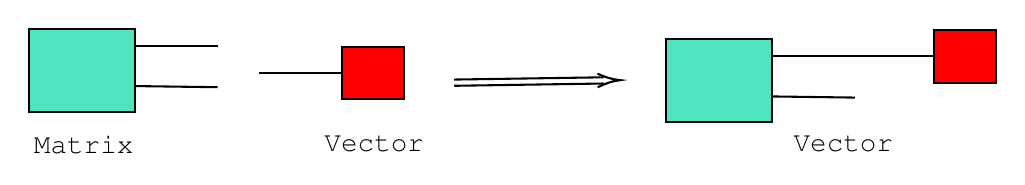
\begin{tikzpicture}[x=0.75pt,y=0.75pt,yscale=-1,xscale=1]
%uncomment if require: \path (0,300); %set diagram left start at 0, and has height of 300

%Shape: Rectangle [id:dp9056942194735556] 
\draw  [fill={rgb, 255:red, 80; green, 227; blue, 194 }  ,fill opacity=1 ] (100,112) -- (151,112) -- (151,152) -- (100,152) -- cycle ;
%Straight Lines [id:da9172659624339214] 
\draw [fill={rgb, 255:red, 80; green, 227; blue, 194 }  ,fill opacity=1 ]   (151,120.18) -- (191,120.18) ;
%Straight Lines [id:da2833939201314972] 
\draw [fill={rgb, 255:red, 80; green, 227; blue, 194 }  ,fill opacity=1 ]   (151,139.63) -- (191,140.18) ;

%Shape: Rectangle [id:dp6422275710126122] 
\draw  [fill={rgb, 255:red, 255; green, 0; blue, 0 }  ,fill opacity=1 ] (251,120.63) -- (281,120.63) -- (281,146) -- (251,146) -- cycle ;
%Straight Lines [id:da9091154996581836] 
\draw [fill={rgb, 255:red, 255; green, 0; blue, 0 }  ,fill opacity=1 ]   (211,133.18) -- (251,133.18) ;

%Straight Lines [id:da6668729559343063] 
\draw    (304.98,136.5) -- (376.98,135.41)(305.02,139.5) -- (377.02,138.4) ;
\draw [shift={(385,136.78)}, rotate = 179.13] [color={rgb, 255:red, 0; green, 0; blue, 0 }  ][line width=0.75]    (10.93,-3.29) .. controls (6.95,-1.4) and (3.31,-0.3) .. (0,0) .. controls (3.31,0.3) and (6.95,1.4) .. (10.93,3.29)   ;
%Shape: Rectangle [id:dp5499160435625281] 
\draw  [fill={rgb, 255:red, 80; green, 227; blue, 194 }  ,fill opacity=1 ] (407,117) -- (458,117) -- (458,157) -- (407,157) -- cycle ;
%Straight Lines [id:da11942666503370314] 
\draw [fill={rgb, 255:red, 80; green, 227; blue, 194 }  ,fill opacity=1 ]   (458,125.18) -- (498,125.18) ;
%Straight Lines [id:da4684372747610551] 
\draw [fill={rgb, 255:red, 80; green, 227; blue, 194 }  ,fill opacity=1 ]   (458,144.63) -- (498,145.18) ;

%Shape: Rectangle [id:dp9126568397813256] 
\draw  [fill={rgb, 255:red, 255; green, 0; blue, 0 }  ,fill opacity=1 ] (536,112.63) -- (566,112.63) -- (566,138) -- (536,138) -- cycle ;
%Straight Lines [id:da5617556659509985] 
\draw [fill={rgb, 255:red, 255; green, 0; blue, 0 }  ,fill opacity=1 ]   (496,125.18) -- (536,125.18) ;


% Text Node
\draw (101,162) node [anchor=north west][inner sep=0.75pt]   [align=left] {{\fontfamily{pcr}\selectfont Matrix}};
% Text Node
\draw (241,162) node [anchor=north west][inner sep=0.75pt]   [align=left] {{\fontfamily{pcr}\selectfont Vector}};
% Text Node
\draw (467,162) node [anchor=north west][inner sep=0.75pt]   [align=left] {{\fontfamily{pcr}\selectfont Vector}};


\end{tikzpicture}
